\documentclass[xcolor=x11names,compress]{beamer}

%% General document %%%%%%%%%%%%%%%%%%%%%%%%%%%%%%%%%%
\definecolor{mygreen}{RGB}{34,139,34}
\definecolor{mypurple}{RGB}{71,60,139}
\definecolor{mybackgr}{RGB}{196,196,196}
\definecolor{myNetworks}{RGB}{0,159,174}
\definecolor{myblue}{RGB}{39,64,139}
\definecolor{mygreyBG}{RGB}{230,230,230}
\definecolor{mytitle}{RGB}{235,235,235}
\definecolor{myNetText}{RGB}{120,119,109}
\definecolor{myred}{RGB}{204,51,51}
\definecolor{myblack}{RGB}{92,92,92}
\definecolor{mygreenBG}{RGB}{152,251,152}
\definecolor{myblueBG}{RGB}{202,225,255}
\definecolor{myredBG}{RGB}{255,48,48}
\definecolor{brownCWI}{RGB}{194,147,86}
\definecolor{redCWI}{RGB}{196,18,48}
\definecolor{textCWI}{RGB}{85,85,85}
\definecolor{skyblueCWI}{RGB}{143,193,193}
\definecolor{mygray}{RGB}{84,84,84}
\usepackage{graphicx}
\usepackage{tikz}
\usetikzlibrary{decorations.fractals}
\usepackage{multicol}
\usepackage{color}
\usepackage{bbold}

\usepackage[utf8]{inputenc}

\usepackage{minted}
\usepackage{amsmath}
\DeclareMathOperator{\Tr}{Tr}

%%%%%%%%%%%%%%%%%%%%%%%%%%%%%%%%%%%%%%%%%%%%%%%%%%%%%%

%% Beamer Layout %%%%%%%%%%%%%%%%%%%%%%%%%%%%%%%%%%
\useoutertheme[subsection=false,shadow]{miniframes}
\useinnertheme{default}
\usefonttheme{serif}
\usepackage{palatino}

%\usepackage{enumitem}

\setbeamerfont{title like}{shape=\scshape}
\setbeamerfont{frametitle}{shape=\scshape}

\setbeamercolor*{lower separation line head}{bg=DeepSkyBlue4} 
\setbeamercolor*{normal text}{fg=black,bg=white} 
\setbeamercolor*{alerted text}{fg=red} 
\setbeamercolor*{example text}{fg=mygreen}
\setbeamercolor*{block text}{fg=mygreen}
\setbeamercolor*{Definition text}{fg=DeepSkyBlue4} 
\setbeamercolor*{structure}{fg=black} 
 
\setbeamercolor*{palette tertiary}{fg=black,bg=black!10} 
\setbeamercolor*{palette quaternary}{fg=black,bg=black!10} 

\renewcommand{\(}{\begin{columns}}
\renewcommand{\)}{\end{columns}}
\newcommand{\<}[1]{\begin{column}{#1}}
\renewcommand{\>}{\end{column}}
%%%%%%%%%%%%%%%%%%%%%%%%%%%%%%%%%%%%%%%%%%%%%%%%%%
\usepackage{amsthm}
\newtheorem{mydef}{Definition}
\usepackage{tcolorbox}

\usetikzlibrary{arrows,positioning} 
\tikzset{
    %Define standard arrow tip
    >=stealth',
    %Define style for boxes
    punkt/.style={
           rectangle,
           rounded corners,
           draw=black, very thick,
           text width=6.5em,
           minimum height=2em,
           text centered},
    % Define arrow style
    pil/.style={
           ->,
           thick,
           shorten <=1pt,
           shorten >=1pt,}
}

\begin{document}


%%%%%%%%%%%%%%%%%%%%%%%%%%%%%%%%%%%%%%%%%%%%%%%%%%%%%%
%%%%%%%%%%%%%%%%%%%%%%%%%%%%%%%%%%%%%%%%%%%%%%%%%%%%%%
\section{\scshape Introduzione}
\begin{frame}
\title{\textbf{Gate per Entanglement:} \\ da catene con 3 spin a reti quantistiche}
%\subtitle{SUBTITLE}
\author{
	Nicola Pancotti\\
	{\it La Sapienza, Università di Roma}}
\date{\includegraphics[width = .45\textwidth]{firstpagepresentation.png}\\
	\vspace{0.1cm}
	\today
}
\titlepage
\end{frame}

%%%%%%%%%%%%%%%%%%%%%%%%%%%%%%%%%%%%%%%%%%%%%%%%%%%%%%
%%%%%%%%%%%%%%%%%%%%%%%%%%%%%%%%%%%%%%%%%%%%%%%%%%%%%%
\begin{frame}{Questo lavoro è stato possibile grazie a:}

%\textbf{\textcolor{DeepSkyBlue4}{\Large}}

\vspace{-1cm}

\begin{multicols}{2}

\begin{center}
\textbf{\textcolor{black}{\large{Prof. Sougato Bose}}}\\
\textcolor{mygray}{University College of London}\end{center}

\columnbreak
\hspace{.5cm}

\vspace{-0.9cm}
\begin{center}
\textbf{\textcolor{black}{\large{Dr. Leonardo Banchi}}}\\ 
\textcolor{mygray}{University College of London}\end{center}

\end{multicols}

\vspace{-.3cm}

$$\&$$

\begin{center}
\textbf{\textcolor{black}{\large{Prof. Paolo Mataloni}}} \\
\textcolor{mygray}{La Sapienza, Università di Roma}\end{center}

\end{frame}

%%%%%%%%%%%%%%%%%%%%%%%%%%%%%%%%%%%%%%%%%%%%%%%%%%%%%%
%%%%%%%%%%%%%%%%%%%%%%%%%%%%%%%%%%%%%%%%%%%%%%%%%%%%%%
\begin{frame}{Introduzione}
\tableofcontents
\end{frame}
%%%%%%%%%%%%%%%%%%%%%%%%%%%%%%%%%%%%%%%%%%%%%%%%%%%%%
\AtBeginSection[]
{
\begin{frame}<beamer>
\frametitle{Outline}
\tableofcontents[currentsection]
\end{frame}
}

%%%%%%%%%%%%%%%%%%%%%%%%%%%%%%%%%%%%%%%%%%%%%%%%%%%%%%
%%%%%%%%%%%%%%%%%%%%%%%%%%%%%%%%%%%%%%%%%%%%%%%%%%%%%%
\section{\scshape Interazioni e Topologia}
\subsection{Possibili configurazioni dell' Hamiltoniana}
\begin{frame}{Il nostro obiettivo...}
\begin{itemize}
  \item \textsc{Ideare nuove Hamiltoniane} 
  \item \textsc{Studiare nuove topologie}
\end{itemize}

\begin{multicols}{2}
\vspace{4cm}
\includegraphics[width = .6\textwidth]{network.pdf}

\normalsize{$$\hat{H} ( \vec{\textsf{J}} ) = \sum_{ij} \sum_{\alpha \beta} \textsf{J}^{\alpha \beta}_{ij} \sigma_i^{\alpha} \sigma_{j}^{\beta}$$}


\columnbreak
\hspace{2.5cm}
\Huge{$$ \rightarrow \hat{H} ( \vec{\textsf{J}} ) $$}

\vspace{-0.7cm}
\begin{minipage}{0.4\textwidth}
\setbeamertemplate{blocks}[rounded][shadow=true]
\setbeamercolor{block body}{fg=black,bg=mytitle}
\begin{block}{\textcolor{blue}{Note}}
\small{\textsc{Il vettore $\vec{\textsf{J}}$ contiene tutte le informazioni che ci interessano}}
\end{block}

\end{minipage}

\end{multicols}


\end{frame}

%%%%%%%%%%%%%%%%%%%%%%%%%%%%%%%%%%%%%%%%%%%%%%%%%%%%%%
%%%%%%%%%%%%%%%%%%%%%%%%%%%%%%%%%%%%%%%%%%%%%%%%%%%%%%
\begin{frame}{Al fine di...}
\begin{itemize}
  \item \textsc{Implementare gate fra i qubit A e B senza rumore} 
  \item \textsc{trovare nuove gate (ed esempio per entanglement)}
  \item \textsc{velocizzare l'attivazione delle gate}
  \item \textsc{sviluppare nuovi algoritmi per trattare questi sistemi}  
  \item \textsc{...}
\end{itemize}
 

\end{frame}

%%%%%%%%%%%%%%%%%%%%%%%%%%%%%%%%%%%%%%%%%%%%%%%%%%%%%%
%%%%%%%%%%%%%%%%%%%%%%%%%%%%%%%%%%%%%%%%%%%%%%%%%%%%%%
\subsection{L'Hamiltoniana e la sua Topologia}
\begin{frame}{Importanza di \textsf{J}}

Contiene informazioni: 
\begin{itemize}
  \item \textsc{se due nodi sono connessi o meno} 
  \item \textsc{l'intensità dell'interazione}
  \item \textsc{il tipo di interazione}
\end{itemize}

\begin{example}[Catena di Spin XX-YY]

\begin{center}
\includegraphics[width = .7\textwidth]{spinchain.png}
\end{center}

\begin{multicols}{2}


\textcolor{myred}{\small{\underline{Evoluzione Quantistica}}} 
\small{$$H(\vec{\textsf{J}}) = \sum_{i=1}^N \textsf{J}^x_{i} \sigma_i^x \sigma_{i+1}^x  +  \textsf{J}^y_{i} \sigma_i^y \sigma_{i+1}^y$$ 
$$\left| \psi_{_{ch}} (t) \right\rangle = \exp \{ - i H(\vec{\textsf{J}}) t  \} \left| \psi_{_{ch}} (0) \right\rangle$$ }

\columnbreak
\vspace{-0.1cm}
\begin{minipage}{0.5\textwidth}
\setbeamertemplate{blocks}[rounded][shadow=true]
\setbeamercolor{block body}{fg=black,bg=mytitle}
\begin{block}{\textcolor{myred}{Question}}
\textit{\small{Esiste un tempo $t^*$ e vettore $\vec{\textsf{J}}$ tali che venga implementata un' \textbf{entangling gate} tra il primo e l'ultimo qubit della catena?}}
\end{block}

\end{minipage}

\end{multicols}


\end{example}


\end{frame}


%%%%%%%%%%%%%%%%%%%%%%%%%%%%%%%%%%%%%%%%%%%%%%%%%%%%%%
%%%%%%%%%%%%%%%%%%%%%%%%%%%%%%%%%%%%%%%%%%%%%%%%%%%%%%
\section{\scshape Teoria}
\subsection{Entangling Gate per catene di spin}
\begin{frame}

\begin{block}{\textcolor{DeepSkyBlue4}{Definizione}}
\textit{$G$ è un' entangling gate se e solo se esiste almeno una matrice densità separabile $\rho_{AB}$ tale che $\rho^{^G}_{AB}= \hat{G} \rho_{AB} \hat{G}^{\dag}$ non è separabile, i.e. entangled.}
\end{block}

\begin{example}
\begin{multicols}{2}
$$CNOT = \begin{pmatrix}1 & 0 & 0 & 0\\0 & 1 & 0 & 0\\0 & 0 & 0 & 1\\0 & 0 & 1 & 0\\\end{pmatrix}$$

\columnbreak

$$
\hat{H} \otimes \mathbb{1} \left| 0  0 \right\rangle = \left| + \right\rangle \left| 0 \right\rangle
$$
$$\downarrow$$
$$
CNOT \left| + \right\rangle \left| 0 \right\rangle = \left| \phi^+ \right\rangle 
$$
\end{multicols}
\vspace{0.08cm}
\begin{center}
\includegraphics[width = .5\textwidth]{CNOTentanglement.png}
\end{center}
\end{example}


\end{frame}


%%%%%%%%%%%%%%%%%%%%%%%%%%%%%%%%%%%%%%%%%%%%%%%%%%%%%%
%%%%%%%%%%%%%%%%%%%%%%%%%%%%%%%%%%%%%%%%%%%%%%%%%%%%%%
\subsection{Likelihood}
\begin{frame}{Likelihood}
\small{$$L_G \left( \vec{\textsf{J}}, \rho_{ab}^k \right) =  \Tr \left\{ G \rho_{ab}^k G^{\dag} \left[  \Tr_{net} \left( e^{-iH(\vec{\textsf{J}})} ( \rho_{ab}^k \otimes \rho_{net} ) e^{iH(\vec{\textsf{J}})} \right) \right]  \right\}$$}


\setbeamertemplate{itemize items}[ball]
\begin{itemize}
  \item $\rho_{ab}^k$ è la matrice densità iniziale dei qubit A e B. Rappresenta uno stato puro e puo' essere sia entangled che separabile.
  \item $\rho_{net}$ è la matrice densità iniziale che descrive il resto della rete. Solitamente $\rho_{net} = \left( \left| 0_{net} \right\rangle \left\langle 0_{net} \right| \right) ^{\otimes (N-2)}$ dove N è il numero di qubit.
\end{itemize}

\end{frame}


%%%%%%%%%%%%%%%%%%%%%%%%%%%%%%%%%%%%%%%%%%%%%%%%%%%%%%
%%%%%%%%%%%%%%%%%%%%%%%%%%%%%%%%%%%%%%%%%%%%%%%%%%%%%%
\subsection{La funzione Fidelity}
\begin{frame}{Fidelity}
Vogliamo misurare quanto bene la nostra dinamica riesce ad implementare una gate $G$. Ci aiuta la seguente funzione

\begin{equation}
\mathcal{F}_G \left( t, \vec{\textsf{J}} \right) = \dfrac{1}{d+1} \left( 1 + \dfrac{1}{d} \sum _{ijkl} G^*_{ik} \mathcal{E}_{ijkl} \left( t \right)  G_{jl} \right)
\end{equation} 

\setbeamertemplate{itemize items}[ball]
\begin{itemize}
  \item $d$ è la dimensione della gate
  \item $\mathcal{E}_{ijkl} = \left\langle i_{ab} \right| \Tr_{net} \left[ e^{-iH(\vec{\textsf{J}})} \left( \left| k_{ab} \right\rangle \left\langle l_{ab} \right| \otimes \left| 0_{net} \right\rangle \left\langle 0_{net} \right| \right) e^{iH(\vec{\textsf{J}})} \right] \left| j_{ab} \right\rangle$
  \setbeamertemplate{itemize items}[default]  
  \begin{itemize}
  	\item $\left| s_{ab} \right\rangle$ è una base
  \end{itemize}
  	
\end{itemize}

\end{frame}


%%%%%%%%%%%%%%%%%%%%%%%%%%%%%%%%%%%%%%%%%%%%%%%%%%%%%%
%%%%%%%%%%%%%%%%%%%%%%%%%%%%%%%%%%%%%%%%%%%%%%%%%%%%%%
\begin{frame}

\setbeamertemplate{blocks}[rounded]
\setbeamercolor{block body}{fg=black,bg=mygreenBG}
\setbeamercolor{block title}{fg=mygreen,bg=white}
\setbeamertemplate{itemize items}[ball]

\begin{columns}[c]
\begin{column}{0.45\textwidth}
\begin{block}{\textsf{\small{Vantaggi}}}
\textsc{Fidelity:}
\begin{itemize}
  \item \footnotesize{E' una media su tutti gli stati iniziali} 
  \item \footnotesize{Dipende solo da $\vec{\textsf{J}}$ e $t$}
\end{itemize}
\textsc{Likelihood:}
\begin{itemize}
  \item \footnotesize{E' abbastanza veloce da calcolare} 
  \item \footnotesize{Ha un controllo più mirato sugli stati iniziali}
\end{itemize}

\end{block}
\end{column}
\hspace{-20pt}

\begin{column}{0.45\textwidth}

\setbeamercolor{block body}{fg=black,bg=myredBG}
\setbeamercolor{block title}{fg=myred,bg=white}

\begin{block}{\textsf{\small{Svantaggi}}}

\textsc{Fidelity:}
\begin{itemize}
  \item \footnotesize{Richiede molto tempo non appena la dimensione del sistema cresce} 
  \item \footnotesize{Nessun controllo sugli stati iniziali}
\end{itemize}
\textsc{Likelihood:}
\begin{itemize}
  \item \footnotesize{SOLO informazioni locali} 
  \item \footnotesize{Lo stato iniziale appartiene ad un insieme molto grande e complicato}
\end{itemize}

\end{block}

\end{column}
\end{columns}


\setbeamertemplate{blocks}[rounded][shadow=true]
\setbeamercolor{block body}{fg=black,bg=white}
\begin{block}{\textcolor{blue}{Si noti}}
\small{$$\mathcal{F}_G \left( \vec{\textsf{J}} \right) = \int d \rho_{ab} \ L_G \left( \vec{\textsf{J}}, \rho_{ab} \right) \sim \lim_{N \rightarrow \infty} \dfrac{1}{N} \sum_{k=1}^N L_G \left( \vec{\textsf{J}}, \rho_{ab}^k \right)$$}
\end{block}

\end{frame}

%%%%%%%%%%%%%%%%%%%%%%%%%%%%%%%%%%%%%%%%%%%%%%%%%%%%%%
%%%%%%%%%%%%%%%%%%%%%%%%%%%%%%%%%%%%%%%%%%%%%%%%%%%%%%
\section{\scshape Gradiente Discendente Stocastico}%
\subsection{SGD classico}
\begin{frame}{Che cos'è Gradiente Discendente Stocastico?}

\begin{columns}[c]
\begin{column}{0.5\textwidth}{\underline{Machine Learning Setup}}
\small{
\begin{enumerate}
  \item \textcolor{myblue}{\textit{Un campione}} $z = (\textbf{x}, y)$
  \item \textcolor{myblue}{\textit{Funzione costo:}} $ \ell (\hat{y}, y)$
  \item \textcolor{myblue}{\textit{Una famiglia di funzioni}} $f \in \mathcal{F}$
  \item \textcolor{myblue}{\textit{cerchiamo $f_{\omega} (\textbf{x})$ che minimizzi}}
  $$\ell (\ f_{\omega} (\textbf{x}), y)$$
\end{enumerate}
}

\textcolor{myred}{Di solito si ha a che fare con medie, quindi è necessario ottimizzare}
$$E_n (f) = \dfrac{1}{n} \sum_{i = 1}^n \ell (\ f_{\omega} (\textbf{x}_i), y_i)$$
\end{column}

\hspace{-10pt}
\vrule{}
\hspace{10pt}
\begin{column}{0.5\textwidth}

\vspace{-0.8cm}

\setbeamercolor{block body}{fg=white,bg=mygray}
\setbeamertemplate{blocks}[rounded]
\begin{block}{}
\vspace{-0.6cm}
$$\omega_{t+1} = \omega_{t} - \gamma \dfrac{1}{n} \sum_{i = 1}^n \nabla_{_{\omega}} Q(\textbf{z}_i, \omega_t)$$

\vspace{-0.6cm}
\Large{$$\downarrow$$}
\vspace{-1.8cm}

$$\omega_{t+1} = \omega_{t} - \gamma_t \nabla_{_{\omega}} Q(\textbf{z}_t, \omega_t)$$

\end{block}


\scriptsize{\textcolor{mygray}{\textcolor{myblue}{La prima} equazione è un algoritmo di Newton \textcolor{myblue}{\emph{Gradiente Discendente}}. 
\vspace{0.1cm}
\\ \textcolor{myred}{La seconda} rappresenta il \textcolor{myred}{\small{\textbf{\emph{Gradiente Discendente Stocastico}}}}}. 

\vspace{0.5cm}

\textit{\textcolor{mygray}{Anzichè calcolare il gradiente di $E_n (f)$  esattamente, ogni step si calcola in base ad un campione, $z_t$, prelevato a random}}}
\end{column}

\end{columns}



\end{frame}

%%%%%%%%%%%%%%%%%%%%%%%%%%%%%%%%%%%%%%%%%%%%%%%%%%%%%%
%%%%%%%%%%%%%%%%%%%%%%%%%%%%%%%%%%%%%%%%%%%%%%%%%%%%%%
\subsection{Due possibili formulazioni (quantistiche)}
\begin{frame}{Due interpretazioni (quantistiche)}


\setbeamertemplate{blocks}[rounded]
\setbeamercolor{block body}{fg=black,bg=mybackgr}
\setbeamertemplate{itemize items}[ball]

\begin{block}{\textsf{\small{Finchè non converge:}}}

\begin{columns}[c]

\begin{column}{0.5\textwidth}
\begin{itemize}
  \item \texttt{\tiny{Generare una matrice densità \\ random $\rho_{1N}$}} 
  \item \tiny{\texttt{Update:} $\mathsf{ \textbf{\textsf{J}} \leftarrow \textbf{\textsf{J}} + \alpha ^{^{- \beta}} \nabla_{\textbf{\textsf{J}}} \  L \left( \textbf{\textsf{J}}, \rho_{1N} \right)}$}
\end{itemize}

\end{column}
\hspace{-50pt}
\vrule{}

\begin{column}{0.5\textwidth}
\begin{itemize}
  \item \texttt{\tiny{Generare una matrice densità random $\rho_{1N}$}} 
  \item \texttt{\tiny{Generare un intero i compreso tra 1 e no. di elementi in $\textbf{\textsf{J}}$}} 
  \item \tiny{\texttt{Update:} $\mathsf{J_i \leftarrow J_i + \alpha ^{^{- \beta}}     \ \dfrac{\partial L \left( \textbf{\textsf{J}}, \rho_{1N} \right)}{\partial J_i}}$}
\end{itemize}

\end{column}
\end{columns}

\end{block}
%\iffalse
\texttt{\scriptsize{\inputminted{python}{presentationSGD.py}
}}
%\fi
\end{frame}

%%%%%%%%%%%%%%%%%%%%%%%%%%%%%%%%%%%%%%%%%%%%%%%%%%%%%%
%%%%%%%%%%%%%%%%%%%%%%%%%%%%%%%%%%%%%%%%%%%%%%%%%%%%%%
\subsection{La scelta dei coefficienti: un problema aperto}
\begin{frame}{La convergenza dello SGD}

\vspace{-0.2cm}

\begin{columns}[c]
\begin{column}{0.35\textwidth}

\setbeamercolor{block title}{fg=white,bg=skyblueCWI}
\setbeamercolor{block body}{fg=black,bg=white}
\setbeamertemplate{blocks}[rounded]

\vspace{0.4cm}

\begin{block}{\textsc{Classicamente}}

\scriptsize\textcolor{textCWI}{La convergenza è garantita per coefficienti che soddisfino
$$\sum_t \gamma_t^2 < \infty$$
$$\sum_t \gamma_t = \infty$$
La velocità è limitata dall'approssimazione del vero gradiente.
}
\end{block}
\end{column}

\hspace{0pt}

\begin{column}{0.35\textwidth}

\setbeamercolor{block title}{fg=white,bg=brownCWI}
\setbeamercolor{block body}{fg=black,bg=white}
\setbeamertemplate{blocks}[rounded]

%\vspace{-1.4cm}

\begin{block}{\small{\textsc{In meccanica quantistica}}}
\scriptsize{
\begin{enumerate}
  \item  \textcolor{textCWI}{Lo spazio di Hilbert è infinito e non numerabile} 
  \item  \textcolor{textCWI}{ I coefficienti dipendono moltissimo dalla \emph{taglia} del sistema}
  \item  \textcolor{textCWI}{Il meglio che abbiamo trovato $$\gamma_t \sim t^{-1/2}$$}
\end{enumerate}
}
\end{block}
\end{column}

\hspace{0pt}

\begin{column}{0.35\textwidth}

\setbeamercolor{block title}{fg=white,bg=redCWI}
\setbeamercolor{block body}{fg=black,bg=white}
\setbeamertemplate{blocks}[rounded]

\vspace{0.2cm}

\begin{block}{\textsc{Un problema aperto}}

\scriptsize{\textcolor{textCWI}{
In teoria $t$ è una variabile continua. Tuttavia, per implementare l'algoritmo, dev'essere discretizzata
\\ \vspace{0.3cm} 
Abbiamo notato che:
}
\begin{itemize}
\item \textcolor{textCWI}{La lunghezza del passo influenza molto la convergenza}
\item \textcolor{textCWI}{Per diverse taglie dobbiamo usare diverse lunghezze!}
\end{itemize}
}
\end{block}
\end{column}

\end{columns}

\begin{columns}[c]

\begin{column}{0.5\textwidth}

\setbeamertemplate{blocks}[rounded][shadow=true]
\setbeamercolor{block body}{fg=black,bg=mytitle}
\begin{block}{\textcolor{myred}{ \small Domanda}}
\textcolor{black}{ \small
Come scegliamo i coefficienti?
\\
Come scegliamo la lunghezza del passo?   
}
\end{block}

\end{column}

\hspace{-10pt}
\vrule{}

\begin{column}{0.5\textwidth}{\small{\textbf{\textsc{\textcolor{skyblueCWI}{Stiamo testando l'Hessiano}}}}}
\vspace{-0.2cm}
$$\omega_{t+1} = \omega_{t} - \gamma_t \Gamma_t \nabla_{_{\omega}} Q(\textbf{z}_t, \omega_t)$$
\footnotesize{\textcolor{textCWI}{\scriptsize $\Gamma_t$ l'inverso della matrice Hessiana. Prende il nome di \emph{SGD al secondo ordine} }}
\end{column}
\end{columns}

\end{frame}

%%%%%%%%%%%%%%%%%%%%%%%%%%%%%%%%%%%%%%%%%%%%%%%%%%%%%%
%%%%%%%%%%%%%%%%%%%%%%%%%%%%%%%%%%%%%%%%%%%%%%%%%%%%%%
\section{\scshape Risultati Numerici}
\subsection{Catene pari e catene dispari}
\begin{frame}{Punto di partenza\footnote{Banchi, Bayat, Verrucchi, Bose, PRL (2011)}}

\vspace{0.3cm}

\begin{columns}[c]
\begin{column}{0.6\textwidth}{\textsc{\textcolor{myNetworks}{Il Modello}}}

\vspace{0.3cm}

\textcolor{myNetText}{
\scriptsize{
$H_{\footnotesize{M}} = \textsf{J} \sum_{n = 1}^N \sigma^x_n \sigma^x_{n+1}  + \sigma^y_n \sigma^y_{n+1} + \lambda \sigma^z_n \sigma^z_{n+1}$
\\
$H_{\footnotesize{I}} = \textsf{J}_0 \sum_{n = 1,N} \sigma^x_n \sigma^x_{n+1}  + \sigma^y_n \sigma^y_{n+1} + \lambda \sigma^z_n \sigma^z_{n+1}
$
} }

\textcolor{myNetText}{
\scriptsize{\\ Nel nostro caso $\lambda = 0$.}
}
\vspace{0.5cm}

\textcolor{myNetText}{
\footnotesize{
Hanno trovato un tempo $t^*$ per una \\ catena di spin per il quale la Fidelity è massima.
}}
\begin{center}
$G_{\footnotesize{AB}} = $
\end{center}

\vspace{-1.2cm}

\begin{center}
\begin{minipage}{0.8\textwidth}
\begin{multicols}{2}
\tiny{

$$
\begin{pmatrix}
1 & 0 & 0 & 0\\
	0 & 0 & 1 & 0\\
	0 & 1 & 0 & 0\\
	0 & 0 & 0 & -1\\
\end{pmatrix}\small{,}
$$
$$N\ ODD$$
\columnbreak

$$
\begin{pmatrix}
1 & 0 & 0 & 0\\
	0 & 0 & i & 0\\
	0 & i & 0 & 0\\
	0 & 0 & 0 & 1\\
\end{pmatrix}
$$
$$
N\ EVEN
$$
}

\end{multicols}
\end{minipage}

\end{center}


\end{column}

\hspace{-20pt}
\vrule{}

\begin{column}{0.6\textwidth}
\scriptsize{\textcolor{redCWI}{
$$\mathcal{F}_G (t) = \int d \psi \left\langle \psi \right| G_{\tiny{AB}}^{\dag} \mathcal{E}_t \left[ \left| \psi \right\rangle \left\langle \psi \right| \right] G_{\tiny{AB}} \left| \psi \right\rangle$$}}
\includegraphics[width = 1\textwidth]{LeoFidPlot.pdf}


\begin{enumerate}[(a)]
\item Evoluzione della funzione Fidelity con $N = 100$ e $\textsf{J}_0 = 0.5\ \textsf{J}$

\item $\mathcal{F}_G (t^*)$ in funzione di N. L'inserto mostra $t^*$ in funzione di N.
\end{enumerate}


\end{column}
\end{columns}


\end{frame}

%%%%%%%%%%%%%%%%%%%%%%%%%%%%%%%%%%%%%%%%%%%%%%%%%%%%%%
%%%%%%%%%%%%%%%%%%%%%%%%%%%%%%%%%%%%%%%%%%%%%%%%%%%%%%

\begin{frame}{SGD in funzione \small{(Likelihood vs Fidelity)}}

\center
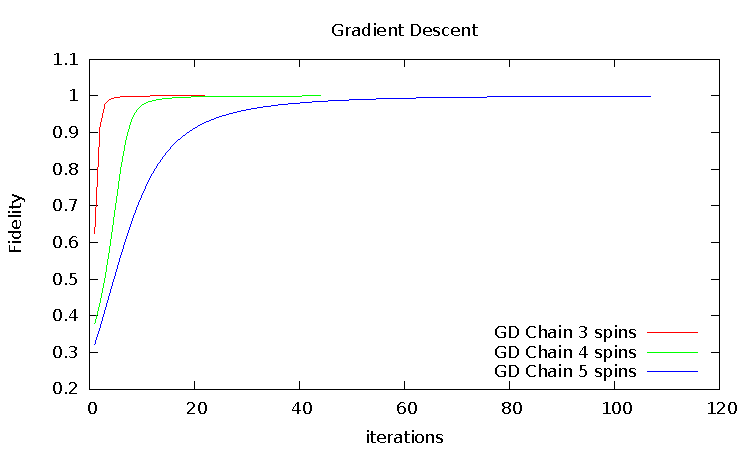
\includegraphics[scale=.4]{GDFidChainXXYYpres2.pdf}
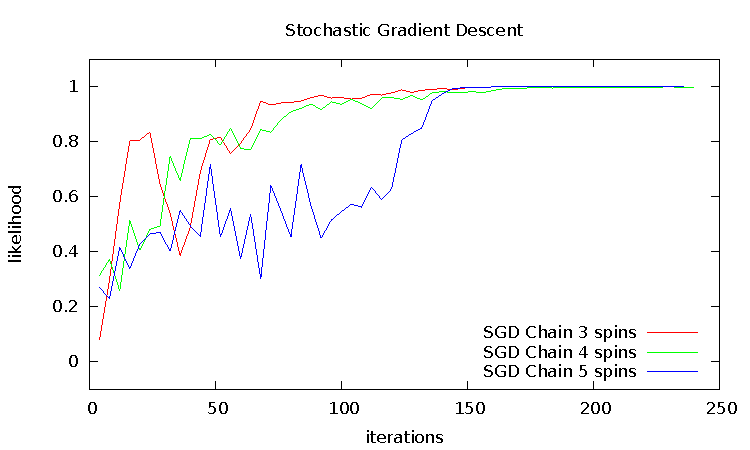
\includegraphics[scale=.4]{SGDChainXXYYpres2.pdf}


\vspace{0.3cm}

\fontsize{7}{9}\selectfont{\textcolor{redCWI}{
\hspace{2.1cm} 3 spins \hspace{2cm} 4 spins \hspace{2cm} 5 spins
\vspace{-0.7cm}
}}

\fontsize{7}{9}\selectfont{
\begin{table}
\begin{tabular}{l | c c | c c | c c}
 & tempo & iterazioni & tempo & iterazioni & tempo & iterazioni\\
\hline
\textcolor{DeepSkyBlue4}{GD Fidelity} & 01' 09.13'' & 22 &  03' 35.20'' & 44 & 11' 41.15'' & 107\\ 
\textcolor{DeepSkyBlue4}{SGD Likelihood} & 00' 12.10'' & 45 & 00' 20.99'' & 36 & 00' 54.14'' & 60 
\end{tabular}
\end{table}
}

\vspace{-0.5cm}

\begin{center}
Si Noti
\end{center}

\vspace{-0.5cm}


\begin{enumerate}
\item \textcolor{myNetText}{\tiny{IL gradiente discendente è un algoritmo \emph{deterministico}. Ovvero, dato uno punto di partenza, la sua destinazione è completamente nota; in molti casi è più proabbile che converga in massimi relativi}}

\item \textcolor{myNetText}{\tiny{Abbiamo provato molte volte a massimizzare la catena a 5 spin con condizioni iniziali random. Alla fine ci siamo arresi ed abbiamo utilizzato l'output dello SGD}}
\end{enumerate}

\end{frame}

%%%%%%%%%%%%%%%%%%%%%%%%%%%%%%%%%%%%%%%%%%%%%%%%%%%%%%
%%%%%%%%%%%%%%%%%%%%%%%%%%%%%%%%%%%%%%%%%%%%%%%%%%%%%%

\subsection{Un'idea sulla topologia}
\begin{frame}{Come possiamo liberarci del \emph{problema} pari/dispari?}

\begin{columns}[c]

\hspace{20pt}



\begin{column}{0.5\textwidth}

\vspace{-.5cm}

\scriptsize{
Ogni gate a due qubit può essere decomposta secondo Cartan:

$$U_{AB} = (U_A \otimes U_B) U_{d} (V_A \otimes V_B) $$

$G_{Odd}$ e $G_{Even}$ sono \emph{localmente equivalenti}; i.e. condividono lo stesso kernel $U_d$.}

\vspace{.7cm}

\setbeamercolor{block body}{fg=black,bg=mygreyBG}
\begin{block}{\textcolor{mygreen}{\textsc{Speravamo}}}

\vspace{-0.5cm}

\scriptsize{ $$G_{Even} = (U_A \otimes U_B) G_{Odd} (U^T_A \otimes U^T_B) $$\\
$\rightarrow$ sono equivalenti a meno di un cambio di base}
\end{block}


\end{column}

\hspace{10pt}

\begin{column}{0.5\textwidth}

\scriptsize{Dato che $\rho (t) = U \rho_0 U^{\dag}$, l'Hamiltoniana più generare è}

\tiny{

$$\downarrow$$

\vspace{-0.4cm}

$$H_{gen} = \sum_{ij} \sum_{\alpha \beta} \textsf{J}^{\alpha \beta}_{ij} \sigma_i^{\alpha} \sigma_{j}^{\beta}$$
}

\scriptsize{Permette tutte le rotazioni e quindi l'implementazione di entrambe le gate}

\vspace{0.4cm}

\setbeamercolor{block body}{fg=black,bg=mygreyBG}
\begin{block}{\textcolor{myred}{\textsc{Tuttavia\footnote{\tiny{Zhang, Vala, Whaley, Sastry, Phys.Rev.A (2003)}}}}}

\vspace{-0.1cm}

\scriptsize{$$G_{Even} = \tiny{\left( \begin{pmatrix} 1 & 0\\ 0 & i\\ \end{pmatrix} \otimes \begin{pmatrix} 1 & 0\\ 0 & i\\ \end{pmatrix} \right) } \cdot G_{_{Odd}} \cdot \mathbb{1}^{\otimes 2}$$\\
$\rightarrow$ che non è un cambio di base.}
\end{block}

\end{column}
\end{columns}


\end{frame}
%%%%%%%%%%%%%%%%%%%%%%%%%%%%%%%%%%%%%%%%%%%%%%%%%%%%%%
%%%%%%%%%%%%%%%%%%%%%%%%%%%%%%%%%%%%%%%%%%%%%%%%%%%%%%
\begin{frame}{\large{\textsl{\underline{\textcolor{brownCWI}{Passando alla rete quantistica}}}}}

\vspace{-0.5cm}

\begin{center}
\begin{tikzpicture}[node distance=1cm, auto,]
 %nodes
 \node (market) {\includegraphics[scale=.09]{7spinEVEN.png}};
 \node[inner sep=3pt,left=3cm of market]
 (formidler) {\includegraphics[scale=.1]{7spinODD.png}};
 % We make a dummy figure to make everything look nice.

 \node[above right= -0.1cm and -2cm of formidler] (g) {\includegraphics[scale=.17]{Equalweights.png}}
 
   edge[pil, bend right=25] (market.west)
   edge[pil, bend left=30] (formidler.east);
\end{tikzpicture}

\end{center}

\vspace{-1cm}

\begin{columns}[c]
\begin{column}{0.5\textwidth}
\begin{center}
\textsc{Odd Gate}
\end{center}
\end{column}

\hspace{1cm}

\begin{column}{0.5\textwidth}
\begin{center}
\textsc{Even Gate}
\end{center}
\end{column}

\end{columns}

\end{frame}

%%%%%%%%%%%%%%%%%%%%%%%%%%%%%%%%%%%%%%%%%%%%%%%%%%%%%%%%%%%%%%%%
%%%%%%%%%%%%%%%%%%%%%%%%%%%%%%%%%%%%%%%%%%%%%%%%%%%%%%%%%%%%%%%%%

\begin{frame}

\setbeamertemplate{blocks}[rounded][shadow=true]
\setbeamercolor{block body}{fg=white,bg=myblack}
\setbeamercolor{block title}{fg=skyblueCWI,bg=myblack}
\setbeamercolor{item}{fg=white}
\setbeamertemplate{itemize items}[ball]

\begin{block}{\textbf{\textsc{Sviluppi possibili}}}

\begin{itemize}
\item \textsl{Studio di reti più grandi e topologie più complesse}
\item \textsl{Trovare nuove rappresentazioni per gate a 3 qubit, e.g. Toffoli}
\item \textsl{Trovare la connessione tra i coefficienti d'apprendimento ed i gradi di libertà del sistema}
\item \textsl{...}
\end{itemize}

\end{block}

\end{frame}

%%%%%%%%%%%%%%%%%%%%%%%%%%%%%%%%%%%%%%%%%%%%%%%%%%%%%%%%%%%%%%%%
%%%%%%%%%%%%%%%%%%%%%%%%%%%%%%%%%%%%%%%%%%%%%%%%%%%%%%%%%%%%%%%%%

\end{document}
